\documentclass[bimj,fleqn]{w-art}
\usepackage{times}
\usepackage{w-thm}
\usepackage[authoryear]{natbib}
% \setlength{\bibsep}{2pt}
% \setlength{\bibhang}{2em}
% \newcommand{\J}{J\"{o}reskog}
% \newcommand{\So}{S\"{o}rbom}
% \newcommand{\bcx}{{\bf X}}
% \newcommand{\bcy}{{\bf Y}}
% \newcommand{\bcz}{{\bf Z}}
% \newcommand{\bcu}{{\bf U}}
% \newcommand{\bcv}{{\bf V}}
% \newcommand{\bcw}{{\bf W}}
% \newcommand{\bci}{{\bf I}}
% \newcommand{\bch}{{\bf H}}
% \newcommand{\bcb}{{\bf B}}
% \newcommand{\bcr}{{\bf R}}
% \newcommand{\bcm}{{\bf M}}
% \newcommand{\bcf}{{\bf F}}
% \newcommand{\bcg}{{\bf G}}
% \newcommand{\bcs}{{\bf S}}
% \newcommand{\bca}{{\bf A}}
% \newcommand{\bcd}{{\bf D}}
% \newcommand{\bcc}{{\bf C}}
% \newcommand{\bce}{{\bf E}}
% \newcommand{\ba}{{\bf a}}
% \newcommand{\bb}{{\bf b}}
% \newcommand{\bc}{{\bf c}}
% \newcommand{\bd}{{\bf d}}
% \newcommand{\bx}{{\bf x}}
% \newcommand{\by}{{\bf y}}
% \newcommand{\bz}{{\bf z}}
% \newcommand{\bu}{{\bf u}}
% \newcommand{\bv}{{\bf v}}
% \newcommand{\bh}{{\bf h}}
% \newcommand{\bl}{{\bf l}}
% \newcommand{\be}{{\bf e}}
% \newcommand{\br}{{\bf r}}
% \newcommand{\bw}{{\bf w}}
% \newcommand{\de}{\stackrel{D}{=}}
% \newcommand{\bt}{\bigtriangleup}
% \newcommand{\bfequiv}{\mbox{\boldmath $\equiv$}}
% \newcommand{\bmu}{\mbox{\boldmath $\mu$}}
% \newcommand{\bnu}{\mbox{\boldmath $\nu$}}
% \newcommand{\bxi}{\mbox{\boldmath $\xi$}}
% \newcommand{\btau}{\mbox{\boldmath $\tau$}}
% \newcommand{\bgamma}{\mbox{\boldmath $\Gamma$}}
% \newcommand{\bphi}{\mbox{\boldmath $\Phi$}}
% \newcommand{\bfphi}{\mbox{\boldmath $\varphi$}}
% \newcommand{\bfeta}{\mbox{\boldmath $\eta$}}
% \newcommand{\bpi}{\mbox{\boldmath $\Pi$}}
% \newcommand{\bequiv}{\mbox{\boldmath $\equiv$}}
% \newcommand{\bvarepsilon}{\mbox{\boldmath $\varepsilon$}}
% \newcommand{\btriangle}{\mbox{\boldmath $\triangle$}}
% \newcommand{\bdelta}{\mbox{\boldmath $\Delta$}}
% \newcommand{\beps}{\mbox{\boldmath $\epsilon$}}
% \newcommand{\btheta}{\mbox{\boldmath $\theta$}}
% \newcommand{\balpha}{\mbox{\boldmath $\alpha$}}
% \newcommand{\bsphi}{\mbox{\boldmath $\varphi$}}
% \newcommand{\bsig}{\mbox{\boldmath $\sigma$}}
% \newcommand{\bfpsi}{\mbox{\boldmath $\psi$}}
% \newcommand{\bfdelta}{\mbox{\boldmath $\delta$}}
% \newcommand{\bsigma}{{\bf \Sigma}}
% \newcommand{\bzero}{{\bf 0}}
% \newcommand{\bpsi}{\mbox{\boldmath $\Psi$}}
% \newcommand{\bep}{\mbox{\boldmath $\epsilon$}}
% \newcommand{\bomega}{\mbox{\boldmath $\Omega$}}
% \newcommand{\bfomega}{\mbox{\boldmath $\omega$}}
% \newcommand{\blambda}{\mbox{\boldmath $\Lambda$}}
% \newcommand{\bflambda}{\mbox{\boldmath $\lambda$}}
% \newcommand{\bfsigma}{\mbox{\boldmath $\sigma$}}
% \newcommand{\bfpi}{{\mbox{\boldmath $\pi$}}}
% \newcommand{\bupsilon}{\mbox{\boldmath $\upsilon$}}
% \newcommand{\obs}{{\rm obs}}
% \newcommand{\mis}{{\rm mis}}
% \theoremstyle{plain}
% \newtheorem{criterion}{Criterion}
% \theoremstyle{definition}
% \newtheorem{condition}[theorem]{Condition}
% \usepackage[]{graphicx}
% \chardef\bslash=`\\ % p. 424, TeXbook
% \newcommand{\ntt}{\normalfont\ttfamily}
% \newcommand{\cn}[1]{{\protect\ntt\bslash#1}}
% \newcommand{\pkg}[1]{{\protect\ntt#1}}
% \let\fn\pkg
% \let\env\pkg
% \let\opt\pkg
% \hfuzz1pc % Don't bother to report overfull boxes if overage is < 1pc
% \newcommand{\envert}[1]{\left\lvert#1\right\rvert}
% \let\abs=\envert

\begin{document}
%\DOIsuffix{bimj.DOIsuffix}
\DOIsuffix{bimj.200100000}
\Volume{52}
\Issue{61}
\Year{2010}
\pagespan{1}{}
\keywords{Evaluation; Imputation; Missing data; Simulation studies;\\ [1pc]
% \noindent \hspace*{-4.2pc} Supporting Information for this article is available from Github, \break \hspace*{-4pc} \underline{github.com/gerkovink/StandardizedEvaluation}.
% } %%% semicolon and fullpoint added here for keyword style
\noindent \hspace*{-4pc} Supporting Information for this article is available online from \\
\hspace*{-4pc} \underline{github.com/gerkovink/StandardizedEvaluation}. 
}  %%% semicolon and fullpoint added here for keyword style

\title[Standardized evaluation]{Towards a standardized evaluation of imputation methodology}
%% Information for the first author.
\author[Oberman]{Hanne I. Oberman\footnote{Corresponding author: {\sf{e-mail: h.i.oberman@uu.nl}}}\inst{,1}} 
\address[\inst{1}]{Departement of Methodology \& Statistics, Padualaan 14, 3584 CH Utrecht, The Netherlands}
%%%%  Information for the second author
\author[Vink]{Gerko Vink\inst{1}}
%%%%  \dedicatory{This is a dedicatory.}
\Receiveddate{zzz} \Reviseddate{zzz} \Accepteddate{zzz} 

\begin{abstract}
Developing new imputation methodology has become a very active field. Unfortunately, there is no consensus on how to perform simulation studies to evaluate the properties of imputation methods. In this paper we propose a move towards a standardized evaluation of imputation methods. To demonstrate the need for standardization, we highlight a set of potential pitfalls that bring forth a chain of potential problems in the objective assessment of the performance of imputation routines. This may lead to sub-optimal use of multiple imputation in practice. Additionally, we suggest a course of action for simulating and evaluating missing data problems.
\end{abstract}



%% maketitle must follow the abstract.
\maketitle          % Produces the title.

%% If there is not enough space inside the running head
%% for all authors including the title you may provide
%% the leftmark in one of the following three forms:

%% \renewcommand{\leftmark}
%% {First Author: A Short Title}

%% \renewcommand{\leftmark}
%% {First Author and Second Author: A Short Title}

%% \renewcommand{\leftmark}
%% {First Author et al.: A Short Title}

%% \tableofcontents % Produces the table of contents.

%%%%%%%%%%%%%%%%%%%%%%%%%%
%% INTRODUCTION
%%%%%%%%%%%%%%%%%%%%%%%%%%

\section{Introduction}

Imputation is a state-of-the-art technique for drawing valid conclusions from incomplete data. The technique has earned a permanent spot in research and policymaking, demonstrated e.g. by the detailed manual created by the National Research Council \citep*{little2012prevention}. Although a top-down enforcement of valid ways to handle missing data is not yet very pronounced, an increasing amount of researchers and data scientists are embracing imputation techniques. After all, the principle of imputation is very intuitive.

The idea behind imputation is to impute (fill in) missing values, to obtain a valid estimate of what could have been. A popular variant is multiple imputation \citep{rubi76}, whereby each missing value is imputed multiple times. The completed data that are thus obtained can be analyzed by standard techniques and, in the case of multiple imputation, the analysis results can be combined into a single inference \citep[using `Rubin's rules'][]{rubi87}. In contrast to ad hoc methods for dealing with missing values (e.g. list-wise deletion, mean imputation, regression imputation, last observation carried forward, indicator method), multiple imputation properly takes into account the sources of uncertainty that are related to the missingness problem. 

The quality of a solution obtained by imputation depends on the statistical properties of the incomplete data and the degree to which an imputation procedure is able to capture these properties when modeling missing values. In general, it holds that modeling missing data becomes more challenging when the amount of missingness increases. However, when (strong) relations in the data are present, the observed parts can hold great predictive power for the models that estimate the missingness. In that case, imputation would be substantially more efficient than the ubiquitous complete case analysis.

When evaluating the statistical properties (and thereby the practical applicability) of imputation methodology, researchers most often make use of simulation studies. In such studies a complete dataset is usually generated from a statistical model, another model is used to induce missingness, and a set of evaluation criteria is postulated to evaluate the performance of one or more missing data methods. However, no golden standard has been established to evaluate imputation routines and, as a result, the validity and aim of the simulation set-ups may differ tremendously from one developer to another. Especially with novel imputation methods being propagated from the fields of machine learning and artificial intelligence, the differences may become more pronounced. Although these promising new methods seem to yield even sharper imputations than now-standard (semi-)parametric imputation methods, the comparison may not be fair due to the simulation setup. 

% [Nowadays there are a lot of imp alg being propagated, esp ai/ml, whose perf often times seems quite promising. But may not be a fair comparison because of the simulation set-up/dev in ai/ml so fast that steps may be skipped. Especially in the field of ML/AI, there are promising new imputation methods, which may yield even sharper imputations than now-standard (semi-)parametric imputation methods]

The purpose of this paper is threefold: First, to raise some concerns with respect to evaluating imputation methodology. These concerns stem from careful consideration with fellow `imputers' and from encounters as a reviewer for statistical journals. Second, to provide imputation methodologists with a suggested course of action when simulating missing data problems. This suggested approach should identify common ground but is in no way intended as an absolute solution. This identifies the third purpose of this paper: discussion. We hope to elicit critical thinking regarding the problems at hand. We are all convinced that our methodology has some merit. But for sake of progress, it would be much more advantageous if the aim of our evaluations would go beyond \textit{proving the point} and would legitimately consider the statistical properties. 


%%%%%%%%%%%%%%%%%%%%%%%%%%
%% PROBLEMS
%%%%%%%%%%%%%%%%%%%%%%%%%%

\section{Why some evaluations should not be trusted}

As of today, there is no consensus on how to perform simulation studies to evaluate the properties of imputation methods. Typically, the developer of a new imputation routine does some tests by simulations, but these tests differ across developers. This brings forth a chain of potential problems in the objective assessment of imputation method performance, within and across studies, which may lead to sub-optimal use of imputation in practice. To demonstrate the broad impact of these problems, we subdivide the problems into the following three distinct categories: problems with data generation, problems with missingness generation, and problems with performance evaluation. We further detail the impact each of these problems may have on the validity of our evaluations. 

%%%%%%%%%%%%%%%%%%%%%%%%%%

\subsection{Data generation problems}

To evaluate the ability of an imputation routine to handle missingness, a form of truth has to be established. Those who perform simulation studies are in the luxury position to establish the truth beforehand by choosing a data generating mechanism. Data generating mechanisms define how a complete dataset is obtained at the start of each simulation repetition. There are two general approaches to generating complete data: (i) model-based simulation, in which data are drawn from a known statistical model or probability distribution, such as the multivariate normal distribution; and (ii) design-based simulation, where data are sampled (with replacement) from a sufficiently large observed set, such as from official registers.

The problem with model-based data generating mechanisms is that a method's performance on simulated data may not translate to empirical data. Real-life data hardly ever follow a given theoretical distribution, so there is no guarantee that simulation results are generalizable. Moreover, data are often generated such that the problem that is being studied is most pronounced, e.g. with consistently high correlations between groups of variables. This results in simulated data that contain such valuable information structures that, no matter what type of missingness would subsequently be induced, the observed parts of the data will still hold much (if not all) of the information about the missing part. Unsurprisingly, the performance of any imputation method will then be evaluated as good. Another threat to the generalizability of model-based simulations is the use of a single model for both data generation and imputation. If data are generated following a model that is also used for imputing the data, the imputation approach will be deemed good (or better than other methods) purely due to the evaluated conditions being in favor of the problem that is studied. Other (unfair) comparative advantages in favor of a certain imputation method may occur due to characteristics of the generated data, such as the number of observations, the number of variables, the variable type(s), and the coherence between variables. In contrast to design-based studies, such characteristics are not always explicit simulation conditions, which may give a false sense of objectivity.

An obvious problem with design-based simulation is that obtaining a large dataset without missing entries can be very challenging. Most real-world data contains at least some missing entries, for which the true underlying missing data model is--by definition--unknown. Therefore, the simulator needs to deal with missingness in \textit{some} way before incomplete empirical data can serve as comparative truth in the simulations. It may seem like an intuitive solution to only draw complete cases from the large dataset, which would indeed yield complete samples. However, there may be inherent differences between cases with and cases without any missing values, due to the unknown missing data model. Only sampling complete cases from the data set may thus result in samples that fail to capture all relevant real-world conditions, which in turn refutes the main reason for using design-based simulation. Another way to deal with missingness in a design-based simulation is to impute the incomplete dataset once, to obtain a single completed dataset to draw samples from. Unfortunately, this practice may favor the imputation method that was used in this initial imputation step throughout any further evaluations. Just to be clear: leaving the missingness as-is and inducing additional missing values to impute could not work here, because we wouldn't have a real and unbiased comparative truth.

After deciding upon a data generating mechanism, another influential--but often overlooked--decision awaits. Simulation studies on missing data methodology have the unique option to exclude sampling variance from their evaluations, and only use the missing data generation procedure as source of Monte Carlo variation. After all, we are interested in the missingness and are not considering the noise induced by the sampling mechanism for evaluation in such studies. Therefore, it is not necessary to take sampling variation into account in order to obtain information about a method's ability to handle the missing data problem, or to objectively compare methods on their ability to correct for missingness \citep[see for a detailed discussion][]{vink14}. The only required change to simulation set-ups is to remove sampling variance from performance evaluation. A lot of published work does not consider this option, while it could have sharpened inconclusive or obfuscated results.  

% Table \ref{table:dgm_truth} displays the source of the comparative truth in simulation studies with and without sampling variance.When deviating conventional pooling rules \citep[cf.][p. 76-77]{rubi87} do not apply. Instead, alternative pooling rules need to be used \citep{raghunathan2003multiple,vink14}. If the sampling variance is not handled correctly, subsequent inferences may be invalid and the simulation results cannot be trusted.


%%%%%%%%%%%%%%%%%%%%%%%%%%

\subsection{Missingness generation problems}

Evaluating imputation methodology requires a missing data problem to be solved. After establishing a comparative truth from a data generating mechanism, some form of missingness therefore has to be induced. Often, however, reports of simulation studies remain vague about the actual missingness conditions under investigation and, even worse, some authors only report something like
\begin{quote}
\textit{We generated missing data following a missing at random missingness mechanism.}
\end{quote}
This should be considered unacceptable as claims about the validity of the imputation inference heavily depend on the simulated missingness conditions, such as missingness mechanisms and missingness patterns. Missingness mechanisms describe the relationship between missing entries and observed data values \citep[generally categorized into MCAR, MAR and MNAR mechanisms c.f.][see Table \ref{table:mech}]{rubi76}.  Missingness patterns concern the location of missing entries across incomplete data \citep[][p. 8]{litt20}. Under this definition, there is a row-wise element to the missingness pattern describing which variables are jointly observed, and a column-wise element encompassing the amount of missingness in the data. 

Even the terminology on missingness generation can be confusing. Does a missingness proportion of 50\% mean that half of the entries in an incomplete dataset are missing, or that half of the rows have at least one missing entry? In this paper, we will henceforth refer to the latter as the proportion of incomplete cases, and keep the term `missingness proportion' restricted to the variable-by-variable interpretation. The distinction between the two concepts, however, is not always clear in the literature, and convoluting the terms may lead to incorrect generalizations because they rarely mean the same (e.g., a proportion of 50\% incomplete cases in bivariate data could translate to a missingness proportion of 25\% in both variables, or one completely observed variable and one with 50\% missingness). Moreover, the value of the actual missingness proportion may be diffusing too. Some studies use only 10\% missingness where other studies push the limits to additionally investigate the performance under missingness proportions of at least 50\%. The inconsistent display of simulation conditions may impact the objectivity of meta-evaluations over imputation methods, as one method's performance may appear to be favorable because of less stringent simulation conditions. This ultimately may lead to statisticians recommending a less efficient method to applied researchers, thereby limiting the efficiency of the imputation approach and unnecessarily lowering the statistical power.

% Remember that missingness is only ignorable under MAR when the parameter of the data is distinct and a-priori independent from the parameter of the missing data process. Under MAR missingness we assume that we may use the observed data to make inferences about the joint (observed and unobserved) data. The dependency of the procedure on the assumption under which we obtain inference is only influenced by the amount of missingness. If there is no missingness--or if there is no data, for that matter--the inference does not depend on the assumption. Alternatively, the validity of assumptions become increasingly important when the missingness increases. Since we control the MAR mechanism, the assumption under which we may solve the missing data problem should hold and it is only fair to assess performance under stringent missingness conditions.

Another aspect of missingness patterns that may misguide evaluations is the complexity of the patterns across variables. It is hardly reasonable to imagine empirical data with only one incomplete variable, yet some simulation studies rely on univariate missingness patterns anyways. Extrapolating simulation results from a specific missing data pattern to more intricate empirical missingness patterns could lead to sub-optimal advice in practice. For example, if a simulator induces missingness in the outcome variable of their analysis model exclusively, they may conclude that list-wise deletion outperforms their imputation method(s). Such a conclusion would, unfortunately, only translate to data that adhere to the same special case \citep[described in][\S 2.7]{fimd}, while biasing inferences in other cases. Another example of a missingness pattern that may inadvertently impose assumptions on generalizations is a monotone pattern \citep[i.e. a pattern with uniformly increasing missingness proportions along variables;][]{litt20}. If a simulator investigates iterative imputation methods under monotone missingness, they might believe that the evaluated imputation algorithms converge instantly, while these methods actually require iteration to produce valid results in all other situations. A final example is multivariate missingness that is generated using step-wise univariate missingness induction. The resulting incomplete data may then not have the intended or expected statistical properties \citep[e.g. skewness;][]{ampute}. This complicates any definitive conclusions about imputation method performance in relation to the data generating mechanism.

% is the   [Other problems with missingness patterns: monotone/univariate vs multivariate, sporadic vs systematic, and univariately generated missing data may not have the expected multivariate patterns.] For example, iterative imputation algorithms converge instantly if there is only one variable with missingness or when the pattern is monotone, but require iteration in all other situations. And very specific missing data patterns may misguide which imputation method prevails in performance: some ad hoc methods are known to yield valid inferences under certain restricted conditions \citep[e.g., list-wise deletion may outperform imputation methods if there is missingness in the outcome variable of the analysis model exclusively][]{fimd}, while biasing inferences in other cases. 
% [Missingness mechanisms paragraphs: 1) definitions of mechanisms (now in table), 2) that MCAR is often ignored, while it's the minimum requirement and reference, and sometimes realistic in practice, 3) that MAR can be generated \textit{spuriously} if the correlation between variables is low,  4) that MNAR is often ignored, while it may be the most realistic in practice, and 5) finally add something about types of M(N)AR (ref Rianne's Dance paper).]
% MCAR missingness: The scenario where the missing values are missing at random and the observed values are observed at random. 
%  the validity of assumptions become increasingly important when the missingness increases.

\begin{table}[tb]
\begin{center}
\caption{Missingness mechanisms. [Add PMAR?]}
\label{table:mech}
\begin{tabular}{lll}
\hline
Mech. & Interpretation and consequences of the mechanism \\
\hline  
MCAR  & Missing completely at random: The probability to be missing is the same for all \\
      & cases. In other words, the missing values are missing at random and the observed \\
      & values are observed at random. \\
MAR   & Missing at random: The probability to be missing is the same within groups of \\
      & cases defined by the observed data only. The essence is that observed relations in \\
      & the data inform the missingness, such that MCAR may be assumed within the \\ 
      & observed groups. \\
MNAR  & Missing not at random: The probability to be missing depends on unobserved \\
      & aspects of the data. The cause of the missingness is unknown and cannot be \\ 
      & inferred from the observed data. This is considered non-ignorable missingness \\
      & \citep[see e.g.][]{rubi76}. \\
\hline
\end{tabular}
\end{center}
\end{table}

Missingness mechanisms are usually assumed to be random (MAR; see Table \ref{table:mech} for definitions). However, the missingness mechanisms that are induced in simulation studies do not necessarily match any true missingness generating mechanisms in incomplete empirical data, nor the mechanisms that are typically assumed when imputing such data. On the one hand, there is MCAR missingness, which may be unlikely as the true missingness generating mechanism, but would yield insightful evaluations in a simulation setting. On the other hand, there is MNAR, which is arguably a quite reasonable source of many real-world missingness scenarios, but is generally ignored except for those evaluations that are specifically targeted at non-ignorable applications. A disconnect between induced missingness, real missingness, and assumed missingness may result in simulation studies that are not as informative as they could be. 

% Out of the three mechanisms , random missingness (MAR) is usually generated for the evaluation of imputation methodology. Missingness mechanisms that are not random (MNAR) and mechanisms that are considered non-ignorable \citep[see e.g.][]{rubi76}, are generally ignored, except for those methods that are specifically targeted at non-ignorable applications. 

% MAR missingness is usually investigated in simulations and assumed in practice. Although MCAR might not reasonably be the true missingness generating mechanism and naturally not typically assumed, the mechanism  can be very insightful in the context of imputation methodology evaluation. By contrast, MNAR

% usually assumed to be random (MAR) or completely random (MCAR). 

MCAR is a necessary simulation condition for evaluating the performance of imputation procedures, yet often omitted. Under MCAR, the statistical properties of the observed data given the missing data are known. Any imputation routine that cannot at least mimic the performance of the observed data inference should be deemed inefficient in the scope of the simulation. If an imputation method is not able to solve the problem (i.e. yield valid inference) under MCAR, the statistical properties of the procedure are not sound. Sadly, the straightforward case of MCAR is often neglected from simulation studies and focus is drawn to the evaluation of MAR mechanisms only. Alternatively, some studies limit their evaluations to MCAR mechanisms only, which in our view may be far too simplistic. 

Although MAR missingness is often considered as simulation condition, the problem of spurious MAR is generally overlooked. With MAR missingness mechanisms, observed relations in the data are used to induce missingness during simulation (e.g. weight is made incomplete based on observed gender to emulate a situation wherein one gender is less likely to disclose their weight). These relations in the observed data may, however, be weak or non-existent. If MAR is induced based on weaker relations in the data, claims for a method's applicability to situations where the missingness is random become less valid. The most extreme example would be when MAR is induced from data without multivariate relations. The inferential implications of the missingness would then mimic those of MCAR, even though the missingness is random. In fact, this would amount to one of the special cases under which complete case analysis would be more efficient than multiple imputation \citep[see e.g.][p. 48]{fimd}: the missingness does not depend on the incomplete variable. This property might be useful in practice, but considering it as a condition to evaluate performance under MAR missingness is useless. 

Inducing a MAR mechanism comes with another issue, namely the type or functional form of the missingness model. Given the simulated data distributions, one random missingness model may be far more disastrous to the observed information than another model \citep{scho18}. This may influence the performance of some (but not necessarily all) imputation routines. For example, inference from hot-deck techniques such as predictive mean matching \citep{little1988missing, rubin1986statistical} may be more severely impacted by large amounts of one-tailed missingness than inference from parametric techniques. It would be a shame to overlook such results due to the focus on a single MAR mechanism.

% Figure \ref{fig:MAR} demonstrates two realizations of missingness mechanisms under MAR mechanisms derived from data with different multivariate relations. 

% \begin{figure}[htb]
% \begin{center}
% \resizebox{\textwidth}{!}{
% 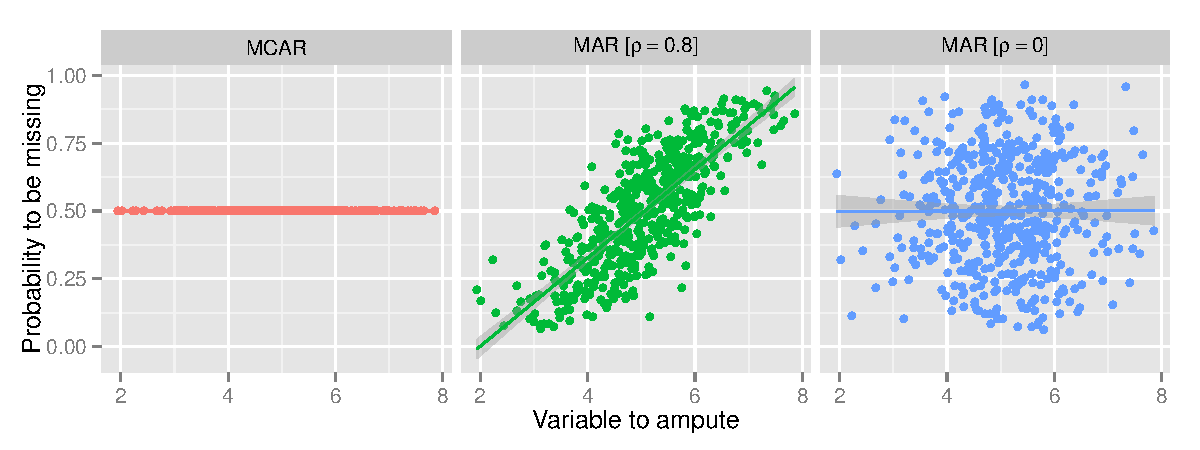
\includegraphics[]{figures/spurious_MAR.pdf}}
% \caption{Three missingness mechanisms that yield approximately 50 percent missingness ($N=500$). Displayed are a MCAR mechanism, a right-tailed MAR mechanism generated from bivariate normal data with correlation $\rho=.8$ and the same MAR mechanism, now generated from bivariate normal data with correlation $\rho= 0$.}
% \end{center}
% \label{fig:MAR}
% \end{figure}
% \vspace*{1pc}

Finally, although one cannot definitively verify if the missingness is random--after all, for every MNAR mechanism there is a MAR mechanism with equal fit \citep{molenberghs2008every}--it can be argued that MNAR is the more likely mechanism for real-life missingness scenarios. As stated, this mechanism is not usually included in evaluations.  % The model--if any--that is used to generate the missingness is usually assumed to be random (MAR) or completely random (MCAR).

% Remember that missingness is only ignorable under MAR when the parameter of the data is distinct and a-priori independent from the parameter of the missing data process. Under MAR missingness we assume that we may use the observed data to make inferences about the joint (observed and unobserved) data. The dependency of the procedure on the assumption under which we obtain inference is only influenced by the amount of missingness. If there is no missingness--or if there is no data, for that matter--the inference does not depend on the assumption. Alternatively, the validity of assumptions become increasingly important when the missingness increases. Since we control the MAR mechanism, the assumption under which we may solve the missing data problem should hold and it is only fair to assess performance under stringent missingness conditions.

%%%%%%%%%%%%%%%%%%%%%%%%%%

\subsection{Evaluation problems}

% The evaluation criteria may depend on the estimand. When descriptive statistics are the goal and when statistical inference would not be of interest, bias of the estimates would still apply, but standard errors are generally ignored. Chances are that for those who focus on descriptive statistical applications, multiple imputation would not be the mode of choice.

% For example, a negligible absolute bias for a parameter for which the true value is zero, would yield infinite bias when relative bias is considered.

The evaluation criteria used to assess imputation performance vary from one simulator to another. This is not surprising as people from different fields could have a different focus on the problem at hand. There are, however, some over-arching issues with assessing imputation method performance. In the first place, evaluations of the imputation-generating process (e.g., an iterative imputation algorithm) are generally left out of simulation study results. In the second place, there are performance measures pitfalls to consider.

Many contemporary imputation techniques rely on iterative algorithms, such as the Gibbs sampler, to generate imputations. As with any iterative algorithm--but especially with imputation algorithms that are critically considered to be possibly incompatible Gibbs samplers \citep[PIGS,][]{li2012imputing}--algorithmic convergence should be carefully evaluated. Unfortunately, there is no universal quantitative method to diagnose non-convergence in iterative imputation algorithms \citep{zhu15, ober21} and the alternative \citep[visual inspection of the imputation algorithm;][]{fimd} is neither efficient nor failproof. As a result, imputation algorithms may be terminated before reaching a stable state, which could yield sub-optimal imputations and under-estimated performance of the method. Moreover, failing to produce stable imputations is not an exclusive quality iterative aimputation algorithms. For example if a method does not yield any imputations at all in a certain simulation repetition (e.g. due to over-parameterization), this can be seen as failure in the imputation-generating process too. 

The evaluation of simulated results relies on the relation between missing data models, imputation models, and analysis models (i.e. the complete data model used to estimate a target or estimand). When an imputation model is able to capture the essence of the true non-response mechanism relative to the analysis model, the models are said to be congenial \citep{meng94}. Congeniality is difficult to diagnose, but ignoring it may yield sub-optimal imputations. Methods to asses the suitability of imputation models and diagnose misfit often rely on visual inspection of the imputations \citep[see e.g.][]{abayomi2008diagnostics, bond16}, which is an infeasible endeavor in many simulation studies. % [All imputation models should be congenial, but this is difficult to test and often ignored. Checks of imputation model fit are often omitted. Ignoring congeniality may yield sub-optimal imputations, which may disadvantage certain methods compared to others. Same goes for convergence: FCS is iterative and requires algorithmic convergence, but this is typically evaluated through visual inspection which is unfeasible in simulation studies. Problems with convergence may be even more severe: some methods do not produce imputations at all for certain conditions, while at other times the imputation algorithm is cut off too soon, and performance will be under-estimated.]  
Therefore, the performance of imputation procedures on distributional properties is often ignored in simulation studies. Even though the estimates on the analysis level may be justified, some methods can yield imputations that may seem completely invalid to applied researchers. For example, one could very accurately estimate average human height by filling in negative values and values that are unrealistically large. While the obtained inference could still be valid under such imputations, the plausibility of the imputed values given the observed data should be under scrutiny. 

% [Add segway between evaluation of imputation and actual performance measures.]
% [Add that simulation aim/target determines which performance measures are relevant to consider, and that the choice of analysis model/estimand can influence the values of these metrics (e.g., focusing on univariate estimates only may favor ad hoc methods).]
% The choice of performance measures may inadvertently distort statistical properties of the imputed data. Developers often only inquire about the `accuracy' (i.e. how well can the method reproduce the original data). [Add RMSE at cell level here?] 

If the goal is inference--not prediction--then the uncertainty about estimates needs to be quantified. A single imputation would then not suffice. The aim of multiple imputation is not to reproduce the data, but to allow for obtaining valid inference given that the data are incomplete. This means that, given the framework provided by \citet{rubi87}, statistical properties such as bias, confidence intervals, and the coverage rate of the confidence intervals should be studied. After all, the 95\% confidence interval should contain the `true' value at least 95 out of 100 times \citep[][p. 591]{neym34}. Merely focusing on distance measures would open the door for invalid inferences.

Some simulators may focus on retrieving the unobserved values, while others study the performance in the context of obtaining efficient predictions or classification. For many outcome-driven imputation task a single valid imputation may suffice. Measures of predictive accuracy or the RMSE (root mean squared error) of predicted values could then serve as sensible evaluation criteria.

%%%%%%%%%%%%%%%%%%%%%%%%%%
%% SOLUTIONS
%%%%%%%%%%%%%%%%%%%%%%%%%%

\section{Suggested course of action}

Standardizing the evaluation of imputation methodology requires simulators--like ourselves--to consider a couple of key aspects in their simulation workflows. Table \ref{table:steps} outlines some suggested steps to adopt. Please note that there is--of course--no `silver bullet' and that we do not claim to present a universally applicable approach. Our suggestions are the accumulated result of scientific literature, research experience, and discussion. For an excellent overview of general best practices for method evaluation by means of simulation, see \citet{morr18}. We recommend adhering to their proposed ADEMP structure (aims, data-generating mechanisms, estimands, methods, performance measures) for planning and reporting simulation studies, but highlight and add some specific recommendations for the evaluation of imputation methodology.


\begin{table}[tb]
\begin{center}
\caption{Steps to consider in imputation simulation studies.}
\label{table:steps}
\begin{tabular}{lll}
\hline
&Step                    & Simulation aspects under consideration \\
\hline  
1&Set scope            & Aim(s), missing data method(s) to evaluate, simulation design \\
2&Obtain truth         & Data generating mechanism(s), estimand(s), sampling variance \\
3&Induce missingness   & Missingness mechanism(s), missing data pattern(s) \\
4&Apply methods        & Imputation model(s), analysis model(s) \\
5&Evaluate imputations & Algorithmic convergence, distributional characteristics, imputation \\
 &                      & model fit \\
6&Evaluate performance & Performance measures, qualitative judgement \\
7&Report               & Text, visualization, checklist, simulation script \\
\hline
\end{tabular}
\end{center}
% \footnotesize{Note. Multiple aspects may be varied across simulation conditions (e.g., using a factorial design with several data generating mechanisms and missingness proportions).}
\end{table}


%%%%%%%%%%%%%%%%%%%%%%%%%%

\subsection{Set scope}

Before setting up a simulation study, the simulator should clearly define the scope of their evaluations. A simulation study aimed at imputation model comparison will typically have a  different design than one aimed at establishing the inferential validity of a single (novel) method. The choice of imputation method(s) under evaluation is naturally intertwined with the simulation study's aims and set-up.

One specific simulation study aim (that we have thus far ignored) is to evaluate the predictive performance of pairs of imputation methods and estimation methods in empirical, incomplete data. These kinds of simulation studies do not start out from a complete data set in which missingness is induced by the simulator. Rather, the evaluations use the observed values of an outcome variable (or target) as the estimand, which is estimated from the incomplete predictor (or feature) space by first imputing the missingness and then applying a prediction method. Pairs of imputation and prediction methods with high predictive accuracy in one or more benchmark data sets are deemed as `good' \citep{liu21}. Note that such a simulation design does not have a `ground truth', so only the comparative performance of methods may be established. We do not recommend this approach if the inferential validity of the imputations is of interest.

% RMSE of the predicted values after imputation and estimation to say something about the comparative performance of the methods. Refer to missing data chapter. In this context, there is no talk of retrieving the `true' but unobserved values at all. The DGM is by definition design-based and there is no sampling variance. The missingness generation step is skipped and the only performance measure that can be used between methods is RMSE and maybe comparison with respect to CCA in terms of bias.]

Some general choices in the simulation set-up to consider at this stage are the simulation design and the number of simulation repetitions. The simulation design should ideally be fully factorial, i.e. varying each simulation condition against all other conditions. There are, for example, known interaction effects between missingness mechanisms and missingness patterns (the validity of the assumed missingness mechanism becomes increasingly important with higher missingness proportions). If there are several imputation method under evaluation, the simulation design should accommodate that each method is applied to each incomplete data set. This is in contrast to a design with as many incomplete data sets as imputation methods in every simulation repetition. Applying all methods to the same incomplete data set is computationally convenient, and minimizes unnecessary variation which makes for fairer comparisons. The number of simulation repetitions may be informed by the required level of precision in the simulation study \citep[e.g. as determined from a maximum tolerable level of uncertainty in terms of a performance measure's Monte Carlo error][]{morr18}. 


%%%%%%%%%%%%%%%%%%%%%%%%%%

\subsection{Obtain truth}

% 1a. choose DGM (if model-based: choose n_obs, n_var, relations between var, var types, etc; if design-based: choose n_obs, missing data handling strategy)
% 1b. decide if sampling variance is needed
% 1c. draw complete sample(s)

The simulator should choose their data generating mechanism(s) in line with the study scope. Model-based data-generating mechanisms have advantages in flexibility and precision, since data are generated from a known statistical model and the true theoretical parameters can be derived. A design-based approach is often used in situations where a probability distribution is not available, or where real-life data structures are of interest. The benefit of design-based simulation is the ability to use real-life observed data structures. 

Estimand(s) or other simulation targets should defined in the context of the study aim and data-generating mechanism. [As a general rule, it would be wise to include one or more multivariate estimands. It is a realistic expectation for imputation methods to yield valid univariate estimates but also to capture multivariable relations in the data. Imputation methods that fail to do so, should not be considered general purpose methods (e.g., mean imputation).]

The comparative truth of the estimand(s) is determined by the choice of data generating mechanism and whether sampling variance is included in the simulation set-up, see Table \ref{table:dgm_truth}. If sampling variance cannot be omitted from the simulation scheme, multiple samples should be drawn from the data generating mechanism (i.e., one sample per simulation repetition, a standard simulation set-up). If sampling variance is not of interest, a single complete data set can be obtained from the data generating mechanism (i.e., one sample for all simulation repetitions). This process is computationally convenient because only a single complete data set has to be considered during all of the simulations. We highly value the additional flexibility that such a simulation set-up offers. Especially in the case of data transformations it can be challenging to derive the true parametric references to evaluate against. Simply using a single generated complete set in which missingness is induced, and evaluating against that generated data set avoids a plethora of procedural problems and computational challenges.
% The simulator should first choose an appropriate data generating mechanism and then decide if sampling variance can be omitted from the simulation scheme to draw one or more samples from the data generating mechanism, respectively.
When deviating from the standard simulation workflow, conventional pooling rules for multiple imputation \citep[cf.][p. 76-77]{rubi87} do not apply. Instead, alternative pooling rules need to be used \citep{raghunathan2003multiple,vink14}.

\begin{table}[tb]
\begin{center}
\caption{Source of the comparative truth in simulation studies.}
\label{table:dgm_truth}
\begin{tabular}{lll}
\hline
               & With sampling variance      & Without sampling variance \\
               & (multiple samples drawn)    & (one sample drawn) \\
\hline  
Model-based simulation   & data-generating model         & single sample \\
Design-based simulation  & sufficiently large data set   & single sample \\
\hline
\end{tabular}
\end{center}
\end{table}

%%%%%%%%%%%%%%%%%%%%%%%%%%

\subsection{Induce missingness}

% 2a. choose missingness mechanism(s): at least consider MCAR, vary MAR types
% 2b. choose missing data pattern(s): introduce non-monotone multivariate missingness
% 2c. choose missingness proportion(s): at least consider 10, 25 and 50\%

Missingness should be induced according to several sets of missing data conditions. We encourage simulators to consider different missingness mechanisms (including missingness types), and different missingness patterns (including missingness proportions). Although not every missingness mechanism is realistically assumed in practice, they can all offer valuable insights as simulation condition. 

First, one should always consider MCAR missingness (see Table \ref{table:mech} for definitions). This mechanism may be used as a reference condition. Valid imputations under MCAR is a minimal requirement for any [multipurpose] imputation method. We also know that, under MCAR, the distribution of imputed values should be equivalent to the distribution of observed values for a given variable, which offers an indication of imputation model (mis)fit. 
% First, one should always consider MCAR missingness [as reference, because all imputation methods should yield valid inference under MCAR and we can use this mechanism to check imputation model fit] %, i.e. the scenario where the missing values are missing at random and the observed values are observed at random. % Under MCAR, the statistical properties of the observed data given the missing data are known and any imputation routine that cannot at least mimic the performance of the observed data inference, should be deemed inefficient in the scope of the simulation. 

Next, missing data should be induced conform a model that is dependent on the observed data (i.e. a MAR mechanism). Arguably, MAR is the most often-assumed mechanism in practice, and should thus be evaluated carefully. A straightforward technique for inducing univariate MAR missingness is described in \citet[][p. 63]{fimd}, generalizations to multivariate MAR missingness can be found in \citet{ampute}, and if the missingness is to be induced in longitudinal data autoregressive MAR models \citep[e.g. cf.][model 2 and model 3]{shara2015randomly} can be useful. It is advisable to investigate varying shapes of MAR missingness to achieve a more realistic indication of the robustness of the imputation performance across the range of random missingness. The effects of different types of MAR mechanisms are described in \citet{scho18}.% Given the simulated data distributions, one random missingness model may be far more disastrous to the observed information than another model. This may influence the performance of some (but not necessarily all) imputation routines. For example, inference from hot-deck techniques such as predictive mean matching \citep{little1988missing, rubin1986statistical} may be more severely impacted by large amounts of one-tailed missingness than inference from parametric techniques. It would be a shame to overlook results due to the focus on a single MAR mechanism. 

Third, a non-ignorable or MNAR mechanism might fall outside many studies' scope, yet could yield informative insights for daily practice. Even if an imputation method is specifically developed with ignorable missingness in mind, chances are that the method will be applied to non-ignorable empirical missingness at some point in time. It would, therefore, be wise to include MNAR missingness in the simulation study just in case, or to perform sensitivity analyses to get an indication of the validity of the obtained inference, given that the assumed missingness mechanism is suspected to be invalid \citep[see e.g.][part 5]{molenberghs2014handbook}.

Apart from the missingness mechanisms, the missingness pattern must be varied--in particular the missingness proportion. Remember that missingness is only ignorable under MAR when the parameter of the data is distinct and a-priori independent from the parameter of the missing data process. Under MAR missingness we assume that we may use the observed data to make inferences about the joint (observed and unobserved) data. The dependency of the procedure on the assumption under which we obtain inference is only influenced by the amount of missingness. If there is no missingness--or if there is no data, for that matter--the inference does not depend on the assumption. Alternatively, the validity of assumptions become increasingly important when the missingness increases. Since we control the MAR mechanism, the assumption under which we may solve the missing data problem should hold and it is only fair to assess performance under stringent missingness conditions. We, therefore, propose to evaluate imputation methodology under 10\%, 25\% and 50\% univariate missingness (see Table \ref{table:prop}). % Although we limit the focus here to ignorable non-response, the suggested proportions are equally applicable to simulations under non-ignorable non-response.


\begin{table}[htb]
\begin{center}
\caption{Suggested univariate missingness proportions.}
\label{table:prop}
\begin{tabular}{lll}
\hline
Prop. & Reasoning for suggested missingness proportion \\
\hline  
10\%  & Depending on the size of the data, this percentage can be considered as a lower \\
      & bound of realistic evaluation. Anything less than 10\% may be of little influence on \\
      & the true data inference. Performance of a missing data method should at least be \\
      & acceptable for most missing data problems. \\ % & \\
25\%  & This is a fair amount of missingness and will, depending on the observed data \\
      & information, have a noticeable influence on the completed data inference. When \\
      & compared to the condition with 10\% missingness, the inference obtained under \\
      & 25\% missingness should be less certain (i.e. confidence/credibility interval width \\
      & should increase), but estimates should still be properly covered and the statistical \\
      & properties of the missing data method should be sound. In practice, at least to our \\
      & at least to my experience in social sciences and official statistics, 25\% \\
      & univariate missingness can easily be considered as a realistic missingness percentage. \\ % & \\
50\%  & Performance under 50\% percent simulated missingness will most likely be impacted \\ 
      & severely. Depending on how the missingness mechanism interacts with the simulated \\
      & data, some imputation techniques may yield estimates that are under-covered such that \\
      & the completed data inference should not be deemed valid anymore. If a method yields \\
      & acceptable inference under 50\% MAR missingness, we can determine that the statistical \\
      & properties of the imputation methodology are sound. \\
\hline
\end{tabular}
\end{center}
\end{table}


%%%%%%%%%%%%%%%%%%%%%%%%%%

\subsection{Apply missing data method(s) and analysis model(s)}

% 3a. Define missing data methods: at least consider complete case analysis as benchmark
% 3b. Choose imputation model parameters: appropriate n_imp and n_it (if applicable), maybe vary predictor matrices?
% 3c. Impute the data
% 3d. Obtain estimates

The imputation method(s) under evaluation should be applied to the generated incomplete data. It is important to choose the imputation model parameters carefully (e.g., number of imputations, number of iterations, regularization, etc.). After imputation, an analysis model may be fitted to estimate the estimand(s).

%[Use CCA as benchmark method: the imputation method should outperform CCA. Choose imputation model parameters carefully (number of imputations, number of iterations if applicable, predictor matrix, regularization if applicable, etc.). Estimate estimand(s) using the analysis model, use correct pooling rules.]

Apart from the imputation method(s), list-wise deletion should be considered as missing data method too. We know the theoretical properties of complete case analysis, which makes the technique useful as a point of departure when evaluating multiple imputation performance. List-wise deletion may therefore serve as a benchmark method: out-performing it should be a minimal requirement for the imputation method(s). %it is wise to evaluate the performance of complete case analysis (aka list-wise deletion) in all simulated conditions.

%%%%%%%%%%%%%%%%%%%%%%%%%%

\subsection{Evaluate imputations}

% 4a. Evaluate imputations: check failed methods, algorithmic convergence (if applicable)
% 4b. Check imputation model fit: anomalies in distributional characteristics, plausibility of imputed values (if requested), PPC

[Some suggested minimal requirements for imputation methods: the absence of algorithmic non-convergence, the imputation model fits the observed parts of the data (PPC), under a MCAR mechanism the imputed values are distributed equivalent to the observed values.]


% = evaluation of imputation generating process
The absence of non-convergence in the imputation models is a minimal requirement for imputation methods. Most contemporary imputation techniques rely on iterative algorithms, such as the Gibbs sampler, where some algorithms are critically considered to be possibly incompatible Gibbs samplers \citep[PIGS,][]{li2012imputing}. The convergence of all iterative algorithms should always be considered and if non-convergence is suspected, the inference resulting from the imputations should not be considered. 

[Distributional characteristics] In practice, the distribution of the incomplete data may differ greatly from the observed data. Under anything but the MCAR assumption, this can be expected. When evaluating imputations, the distributional shapes should be checked and diagnostic evaluations should be performed \citep[see][for a detailed overview of diagnostic evaluation for multivariate imputations]{abayomi2008diagnostics}. When anomalies are found, and if the imputation method is valid, there should be an explanation, especially in the controlled environment of a properly executed simulation study. 

The fit of the imputation model may be verified with the help of a posterior predictive check \citep[PPC][]{nguy17, zhao22}. A PPC in the context imputation methodology could be the over-imputation of observed data values. The reasoning is that if the over-imputed values have  equivalent statistical properties to the true data values, the imputation model fits the observed part of the incomplete data well. We might then assume that the imputation model would be able to produce good imputations for missing values as well. 

[Plausibility of the imputed values] Plausible imputations--imputations that could be real values if they had been observed--are not a necessary condition for obtaining valid inference. However, in practice, especially when the imputer and the analyst are different persons, plausible imputations may be a desired property. One would prefer an imputation technique to yield both valid inference and plausible imputations. It should be studied if an imputation method is prone to deliver such impractical results, and if so, under what conditions. When evaluating imputation routines, the evaluator should mention whether the routine is prone to deliver implausible values. 



%%%%%%%%%%%%%%%%%%%%%%%%%%

\subsection{Evaluate performance}

% 4c. Apply performance measures: at least consider bias, coverage, CI length, if applicable also RMSE (at prediction and/or cell level)
% fraction of missing information (= model parameter), variance inflation

[Some suggested minimal requirements for imputation methods: the method yields valid inference under MCAR, the method performs equally well or better than complete case analysis (i.e. performance after list-wise deletion).]

% sim perf and model perf
[The evaluation criteria may depend on the estimand. When descriptive statistics are the goal and when statistical inference would not be of interest, the bias of the estimates would still apply, but standard errors are generally ignored. Chances are that for those who focus on descriptive statistical applications, multiple imputation would not be the mode of choice.] 

In general, we would say that each multiple imputation routine should be evaluated on at least the following points:
 (i) Bias: Results should preferable be unbiased. However, the way bias is considered can greatly influence the interpretation of the results. For example, a negligible absolute bias for a parameter for which the true value is zero would yield infinite bias when relative bias is considered. The way bias is computed should therefore be carefully chosen and described. 
(ii) Coverage: Coverage of a 95\% interval should in theory be $\geq 95$, where a coverage rate of 95\% would be most efficient. Under-coverage (when estimation is too liberal) may be an indication of invalid inference, while over-coverage (when estimation is too conservative) tells us that efficiency could still be gained. 
(iii) Interval width: The way the confidence interval is calculated should be described. Wider intervals are associated with more uncertainty and the more narrow interval that is still properly covered indicates a sharper inference. However, inference from a wider interval that is properly covered is to be considered more valid when compared to a more narrow interval that is not properly covered anymore. 
% [Add RMSE at cell level and at prediction level (if applicable).]

Last, when the evaluator is on the verge of drawing conclusions about the performance of the imputation routine, the performance should be carefully qualified. Comparing the performance of an imputation routine given a population (or true) parameter allows for quantitative evaluation. However, in order to pose qualitative statements about the performance on simulated conditions, comparative methodology is required. For example, when claiming that imputation performance is unacceptable when deviations from normality become rather stringent, such performance is highly dependent on the simulation conditions that are used. For a well-balanced judgment about the severity of the performance drop, comparative simulations with e.g. nonparametric models should be executed. A method may perform badly, but if it still outperforms every other approach, it may yet be of great practical relevance.

It could be convincing to demonstrate a method's applicability to real-world missing data problems. This can, for example, be achieved by obtaining and imputing a fully observed set of variables, wherein the missingness is mimicked from a similar, incomplete set. Alternatively, an incomplete set could be obtained and truth could be established by removing the incomplete cases from the data. However, the real-world missingness would then be omitted.


%%%%%%%%%%%%%%%%%%%%%%%%%%

\subsection{Report}

[Be explicit in choices. Describe the simulation textually, use pseudo-code, a flowchart, visualize missingness and simulation results. For example, the used missingness mechanism should be detailed, either graphically or written as a function of the data. And the procedure to generate missing data is often insufficiently described in resulting publications. Fill in the following checklist (in appendix).]


%%%%%%%%%%%%%%%%%%%%%%%%%%
%% DISCUSSION
%%%%%%%%%%%%%%%%%%%%%%%%%%

\section{Discussion}

This manuscript aims to establish a common ground for the evaluation of imputation routines. Such a common ground would be the basis of a standardized evaluation. This would allow for fairer and more efficient comparisons between imputation techniques. Ultimately, it would be desirable to evaluate every imputation routine against the same standardized set in order to quantify the statistical properties across imputation routines. If properly executed, this would allow for careful matching of imputation methodologies to new missing data problems. 


%%%%%%%%%%%%%%%%%%%%%%%%%%
%% APPENDICES
%%%%%%%%%%%%%%%%%%%%%%%%%%

\begin{acknowledgement}
We thank the Amices team for the fruitful discussions.
\end{acknowledgement}
\vspace*{1pc}

\noindent {\bf{Conflict of Interest}}

\noindent {\it{The authors have declared no conflict of interest.}}

\section*{Appendix}

\subsection*{A.1.\enspace Checklist for the evaluation of imputation methodology}

1. Set-up

- aim

- target/estimand + analysis model

- precision level + number of simulations

2. Data generation

- model vs design based

- sampling variance

- number of observations

- number of variables

- data types + structures (e.g. clustering/time-series)

- coherence between variables

3. Missingness generation

- missingness mechanism + type (if applicable)

- missingness patterns (rows = univariate/multivariate; columns = proportion)

4. Missing data methods

- imputation methods + list-wise deletion

- imputation method parameters (e.g. number of imputations)

- imputation model parameters (e.g. predictor matrix)

5. Imputation evaluation

- imputation process (e.g. non-convergence)

- imputation model fit (PPC)

- distribution of imputations (e.g. plausibility)

- imputation accuracy (e.g. RMSE at cell level)

6. Performance evaluation

- statistical properties (e.g. confidence validity)

- comparative performance (e.g. RMSE of predictions)

7. Report


%%%%%%%%%%%%%%%%%%%%%%%%%%
%% REFERENCES
%%%%%%%%%%%%%%%%%%%%%%%%%%
\bibliography{bibliography}
\bibliographystyle{apalike}

% \begin{thebibliography}{10}
% \bibitem[Bauer and Bauer(1994)Bauer, P. and Bauer, M.M.]{bib1}Bauer, P. and Bauer, M. M. (1994). Testing equivalence simultaneously for location and dispersion of two normally distributed populations. \textit{Biometrical Journal} \textbf{36}, 643--660.
% \bibitem[Farrington, C. P. and Andrews, N. (2003)]{bib2}Farrington, C.P. and Andrews, N. (2003). Outbreak detection:
% Application to infectious disease surveillance. In: Monitoring the Health of Populations (eds. R. Brookmeyer and D. F. Stroup), Oxford University Press, Oxford,\break 203--231.
% \bibitem[Rencher(1998)Rencher, A.C.]{bib3}Rencher, A. C. (1998). \textit{Multivariate Statistical Inference and Applications}. Wiley, New York. 
% \end{thebibliography}
% \newpage
% \phantom{aaaa}
\end{document}